\chapter{Proposed Architecture}\label{ch:proposed_architecture}
\epigraph{\textit{\normalsize “Artificial intelligence, in fact, is obviously an intelligence transmitted by conscious subjects, an intelligence placed in equipment.”}}{\textit{ \normalsize Pope Benedict XVI}}

The generator will use noise as input to generate faces. We will use random data as this noise. This ensures the data is unique and across the spectrum while retaining a normal distribution.
\par\bigskip

The CapsNet making up the discriminator consists of a small convolutional network to convert low level data in the form of pixels into an artifact called "pose". These poses can be anything, like nose, ear, eye, etc. These poses are then passed on as input to the later lower layers consisting of components called Capsules. A capsule is analogous to the human brain containing different modules to handle different tasks. The brain has a mechanism to route the information among the modules, to reach the best modules that can handle the information.
\par\bigskip

A capsule is a nested set of neural layers. Each capsule is able to handle one particular pose and communicate its calculation to other capsules which can use that calculation. This calculation is in the form of a probability prediction of the current pose that takes place in its logistic unit. This working is fundamentally different from convolutional networks, which utilizes Max Pooling. Max pooling selects the most active input node from the next layer to pass on the information. CapsNet on the other hand selects the next capsule based on which capsule would be capable of handling that information. This is called Dynamic routing. This results in invariance of information to the position and orientation of features in an object while ignoring the invariance in very low level features as, at the pixel level, this does not matter.
\par\bigskip

\section{Generator} % (fold)
\label{sec:generator}
We use a deep convolutional generator model, which is similar to what DCGAN uses as generator. It starts with a latent vector or noise of shape 100 which connects to a densely connected neural layer. We then use Reshape layer which reshapes it to an (8, 8, 128) matrix and which is then sent to the batch normalization layer. We later perform up-sampling by using DeConv (De-Convolutional layer: transposed convolutional layer) layer. DeConv layer is internally implemented by an up-sampling layer and a convolutional layer. We perform DeConv two more times to get the shape of the image as expected, which should be (64, 64, 3), which stands for a 64x64 RGB image.
\begin{figure}[H]
\centering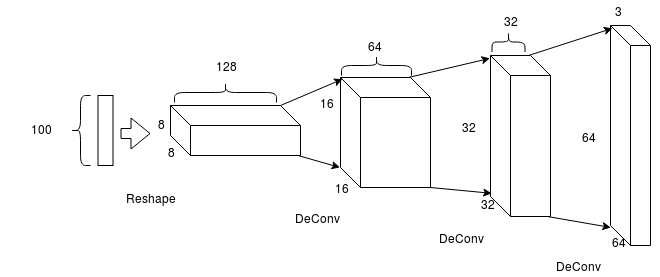
\includegraphics[width=1\textwidth]{images/Generator.png}
\caption{Generator architecture}
\label{fig:generator}
\end{figure} 

% section generator (end)


\section{Discriminator} % (fold)
\label{sec:discriminator}
\begin{figure}[H]
\centering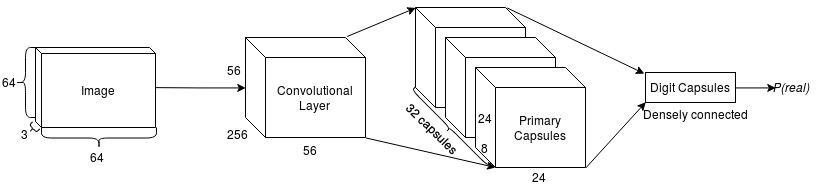
\includegraphics[width=1\textwidth]{images/Discriminator.png}
\caption{Discriminator architecture}
\label{fig:discriminator}
\end{figure} 
The discriminator in the original models is replaced by our modification of CapsNet. We use a binary classifier CapsNet to distinguish between real and fake images. 

\par\bigskip
The CapsNet has 2 parts: encoder and decoder. The first 3 layers are encoder, and the second 3 are decoder:

Layer 1. Convolutional layer
Layer 2. PrimaryCaps layer
Layer 3. DigitCaps layer
Layer 4. Fully connected \#1
Layer 5. Fully connected \#2
Layer 6. Fully connected \#3

In our implementation, we do not use the decoder layers as we do not need the reconstruction aspects of the network for classification. Hence only the encoder layers are used.
\par\bigskip
The encoding part of the network takes as input a digital image of 64x64 and learns to encode it into a vector of 16 dimensions of instantiation parameters, this is where the capsules do their job. The output of the network during prediction is a 10-dimensional vector of the lengths of the DigitCaps' outputs.

% Discriminator image

\subsection{Layer 1: Convolutional Layer} % (fold)
\label{sub:layer_1_convolutional_layer}
\noindent Input: 64x64 image (three color channel).
\\Output: 56x56x256 tensor.
\\Number of parameters: 62464.

\par\bigskip The work of the convolutional layer consists of detecting the basic functions in the 2D image. In the CapsNet system, the convolutional layer has 256 kernels of size 9x9x1 and stride of 1, followed by the activation function, ReLU. To calculate the number of parameters, we must also remember that each kernel in a convolutional layer has 1 bias term. Therefore, this layer has (9 x 9 x 3 x 256 + 256 =) 62464 trainable parameters in total.

% subsection layer_1_convolutional_layer (end)

\subsection{Layer 2: PrimaryCaps Layer} % (fold)
\label{sub:layer_2_primarycaps_layer}
\noindent Input: 56x56x256 tensor.
\\Output: 24x24x8x32 tensor.
\\Number of parameters: 5308672.

\par\bigskip This layer has 32 primary capsules whose job is to take basic features detected by the convolutional layer and produce combinations of the features. The layer has 32 “primary capsules” that are very similar to convolutional layer in their nature. Each capsule applies eight 9x9x256 convolutional kernels to the 56x56x256 input volume and therefore produces 24x24x8 output tensor. Since there are 32 such capsules, the output volume has shape of 24x24x8x32. Doing calculation similar to the one in the previous layer, we get (9 x 9 x 256 x 256 + 256 =) 5308672 trainable parameters in this layer.

% subsection layer_2_primarycaps_layer (end)

\subsection{Layer 3: DigitCaps Layer} % (fold)
\label{sub:layer_3_digitcaps_layer}
\noindent Input: 24x24x8x32 tensor.
\\Flattened to: 147456
\\Output: 1x1 matrix.
\\Number of parameters: 1497600.

\par\bigskip We have a 3 hidden-layer densely connected neural network which takes the flattened input to give a binary classification output of 1x1. Each hidden layer consists of 160 neurons. From the flattened input we get the input of size 147456 which is connected densely to the first hidden layer. Thus the weights in the first layer turn out to be (147456 x 160 + 160 =)  23593120 in number. The first hidden layer is connected to the second hidden layer densely, similarly the second and the third. Therefore there are (160 x 160 + 160 =) 25760 trainable parameters for the second and third hidden layers. 
\par\bigskip The last last hidden layer is connected to a output layer with one neuron, which essentially gives the binary classification result. Its parameters are (160 x 1 + 1 =) 161 in number. 
% subsection layer_3_digitcaps_layer (end)

% section discriminator (end)



% _________________________________________________________________
% Layer (type)                 Output Shape              Param #   
% =================================================================
% dense_5 (Dense)              (None, 8192)              827392    
% _________________________________________________________________
% reshape_1 (Reshape)          (None, 8, 8, 128)         0         
% _________________________________________________________________
% batch_normalization_3 (Batch (None, 8, 8, 128)         512       
% _________________________________________________________________
% up_sampling2d_1 (UpSampling2 (None, 16, 16, 128)       0         
% _________________________________________________________________
% conv2d_1 (Conv2D)            (None, 16, 16, 128)       147584    
% _________________________________________________________________
% activation_1 (Activation)    (None, 16, 16, 128)       0         
% _________________________________________________________________
% batch_normalization_4 (Batch (None, 16, 16, 128)       512       
% _________________________________________________________________
% up_sampling2d_2 (UpSampling2 (None, 32, 32, 128)       0         
% _________________________________________________________________
% conv2d_2 (Conv2D)            (None, 32, 32, 64)        73792     
% _________________________________________________________________
% activation_2 (Activation)    (None, 32, 32, 64)        0         
% _________________________________________________________________
% batch_normalization_5 (Batch (None, 32, 32, 64)        256       
% _________________________________________________________________
% up_sampling2d_3 (UpSampling2 (None, 64, 64, 64)        0         
% _________________________________________________________________
% conv2d_3 (Conv2D)            (None, 64, 64, 32)        18464     
% _________________________________________________________________
% activation_3 (Activation)    (None, 64, 64, 32)        0         
% _________________________________________________________________
% batch_normalization_6 (Batch (None, 64, 64, 32)        128       
% _________________________________________________________________
% conv2d_4 (Conv2D)            (None, 64, 64, 3)         867       
% _________________________________________________________________
% activation_4 (Activation)    (None, 64, 64, 3)         0         
% =================================================================
% Total params: 1,069,507
% Trainable params: 1,068,803
% Non-trainable params: 704
% \begin{lstlisting}[basicstyle=\scriptsize,]
% __________________________________________________________________________________________________
% Layer (type)                    Output Shape         Param #     Connected to                     
% ==================================================================================================
% input_1 (InputLayer)            (None, 64, 64, 3)    0                                            
% __________________________________________________________________________________________________
% conv1 (Conv2D)                  (None, 56, 56, 256)  62464       input_1[0][0]                    
% __________________________________________________________________________________________________
% leaky_re_lu_1 (LeakyReLU)       (None, 56, 56, 256)  0           conv1[0][0]                      
% __________________________________________________________________________________________________
% batch_normalization_1 (BatchNor (None, 56, 56, 256)  1024        leaky_re_lu_1[0][0]              
% __________________________________________________________________________________________________
% primarycap_conv2 (Conv2D)       (None, 24, 24, 256)  5308672     batch_normalization_1[0][0]      
% __________________________________________________________________________________________________
% primarycap_reshape (Reshape)    (None, 18432, 8)     0           primarycap_conv2[0][0]           
% __________________________________________________________________________________________________
% primarycap_squash (Lambda)      (None, 18432, 8)     0           primarycap_reshape[0][0]         
% __________________________________________________________________________________________________
% batch_normalization_2 (BatchNor (None, 18432, 8)     32          primarycap_squash[0][0]          
% __________________________________________________________________________________________________
% flatten_1 (Flatten)             (None, 147456)       0           batch_normalization_2[0][0]      
% __________________________________________________________________________________________________
% uhat_digitcaps (Dense)          (None, 160)          23593120    flatten_1[0][0]                  
% __________________________________________________________________________________________________
% softmax_digitcaps1 (Activation) (None, 160)          0           uhat_digitcaps[0][0]             
% __________________________________________________________________________________________________
% dense_1 (Dense)                 (None, 160)          25760       softmax_digitcaps1[0][0]         
% __________________________________________________________________________________________________
% multiply_1 (Multiply)           (None, 160)          0           uhat_digitcaps[0][0]             
%                                                                  dense_1[0][0]                    
% __________________________________________________________________________________________________
% leaky_re_lu_2 (LeakyReLU)       (None, 160)          0           multiply_1[0][0]                 
% __________________________________________________________________________________________________
% softmax_digitcaps2 (Activation) (None, 160)          0           leaky_re_lu_2[0][0]              
% __________________________________________________________________________________________________
% dense_2 (Dense)                 (None, 160)          25760       softmax_digitcaps2[0][0]         
% __________________________________________________________________________________________________
% multiply_2 (Multiply)           (None, 160)          0           uhat_digitcaps[0][0]             
%                                                                  dense_2[0][0]                    
% __________________________________________________________________________________________________
% leaky_re_lu_3 (LeakyReLU)       (None, 160)          0           multiply_2[0][0]                 
% __________________________________________________________________________________________________
% softmax_digitcaps3 (Activation) (None, 160)          0           leaky_re_lu_3[0][0]              
% __________________________________________________________________________________________________
% dense_3 (Dense)                 (None, 160)          25760       softmax_digitcaps3[0][0]         
% __________________________________________________________________________________________________
% multiply_3 (Multiply)           (None, 160)          0           uhat_digitcaps[0][0]             
%                                                                  dense_3[0][0]                    
% __________________________________________________________________________________________________
% leaky_re_lu_4 (LeakyReLU)       (None, 160)          0           multiply_3[0][0]                 
% __________________________________________________________________________________________________
% dense_4 (Dense)                 (None, 1)            161         leaky_re_lu_4[0][0]              
% ==================================================================================================
% Total params: 29,042,753
% Trainable params: 29,042,225
% Non-trainable params: 528
% __________________________________________________________________________________________________
% \end{lstlisting}
